\section{Desarrollo}

\subsection{Manejo del Header de una Imagen}

	Como se sabe, hay diferentes formatos para guardar la informaciond e una imagen, etre ellos puede ser \textit{.jpg},\textit{png},\textit{etc}. Para el anaisis del header de la imagen, se fijo dicho formato eligiendo el formato \textit{bmp} de \textit{24-bytes}. En la figura (\ref{fig:formato}), se observa que el formato consiste en 3 encabezados correspondiente sobre la información del archivo, la información de colores y sobre la información de los datos. Luego tiene un vector que se corresponde a los datos. 

	La modificación del header se hizo a través de una imagen patrón conocida como \textit{Lenna} en formato \textit{.bmp}. La imagen se muestra en la figura (\ref{fig:lenna}) tine una altura de \textit{512} y un ancho de \textit{512}.
	
\begin{figure}[H]
	\centering
	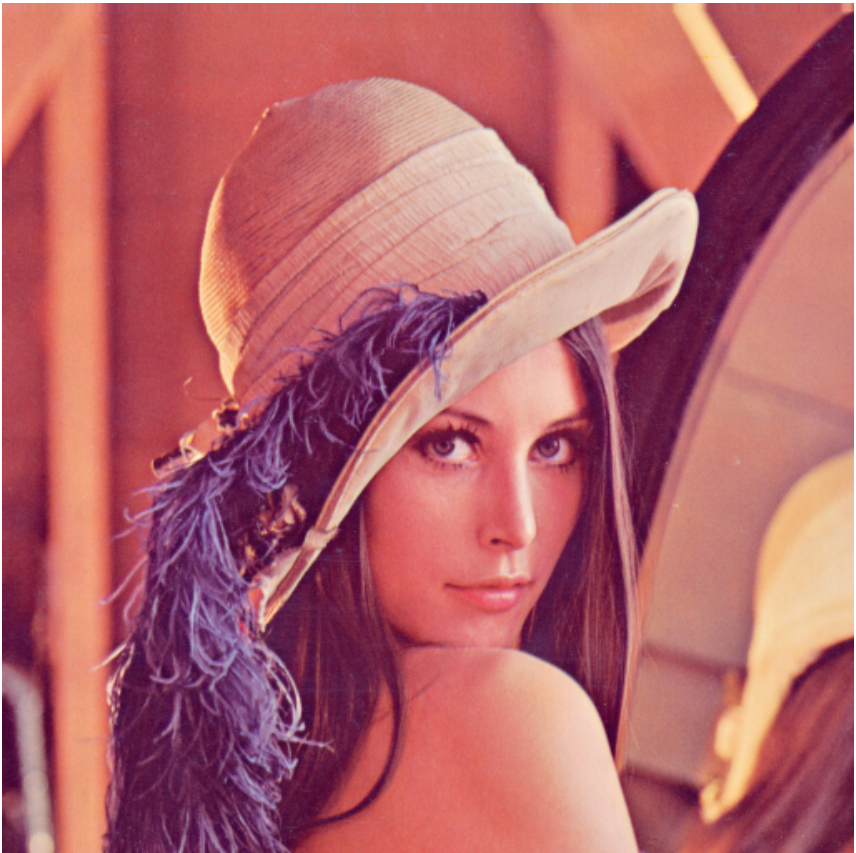
\includegraphics[scale=0.5]{imagenes/lenna.png}]
	\caption{Imagen patron usada en los trabajos practicos de \textit{512x512}\label{fig:lenna}}
\end{figure}
	

\begin{figure}[H]
	\centering
	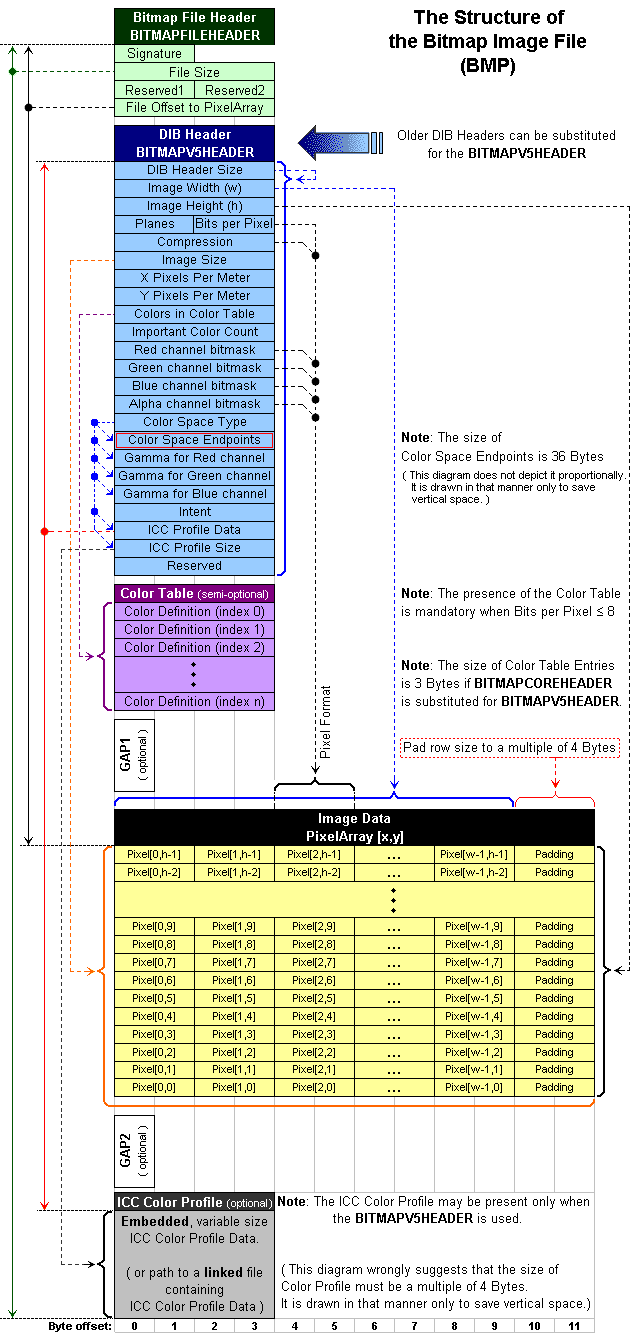
\includegraphics[scale=0.5]{imagenes/BMPfileFormat.png}]
	\caption{Encabezado de una imagen con formato \textit{bmp}	\label{fig:formato}}
\end{figure}


\section{Modificación del Ancho y el Alto de la imagen}

	En este punto se agarro la imagen patrón y se modifico los valores de la altura y el ancho de la imagen observando diferentes resultados, se comenzó reduciendo y multiplicando la altura y el ancho obteniendo lo siguiente

\begin{figure}[H]
	\centering
	\subfigure[Altura multiplicada por 2]{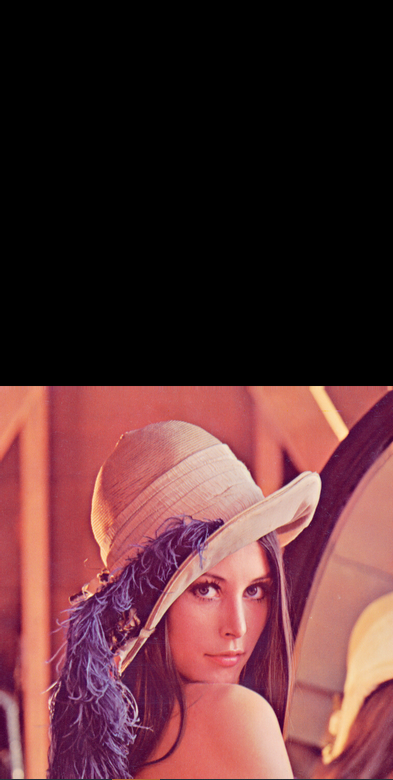
\includegraphics[scale=0.5]{imagenes/Hmul2.png}]}
		\subfigure[Altura dividida por 2]{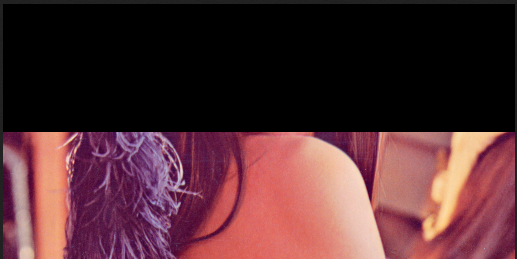
\includegraphics[scale=0.5]{imagenes/Hdiv2.png}]
	}
	\caption{Resultado de cambiar la altura de la imagen.}
\end{figure}	

\begin{figure}[H]
	\centering
	\subfigure[Ancho multiplicado por 2]{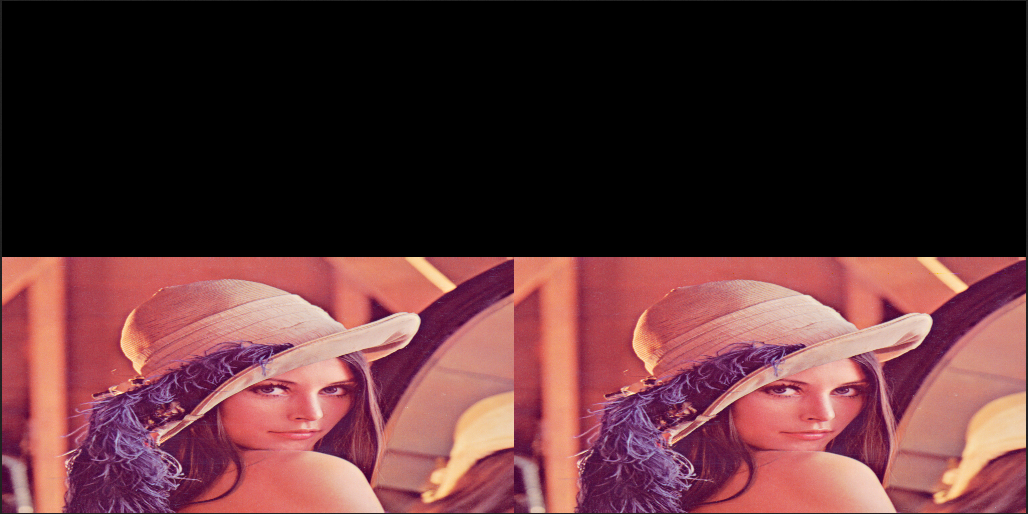
\includegraphics[scale=0.5]{imagenes/Wmul2.png}]}
		\subfigure[Ancho dividido por 2]{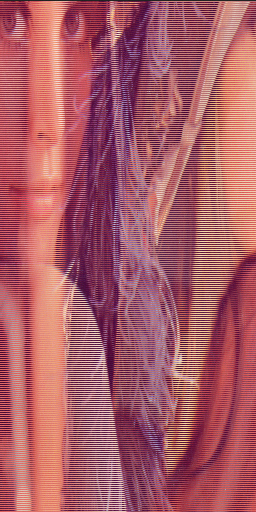
\includegraphics[scale=0.5]{imagenes/Wdiv2.png}]
	}
	\caption{Resultado de cambiar el ancho de la imagen.}
\end{figure}	

	Mirando el análisis de la modificación del header se decidió, cambiar el alto y el ancho al mismo tiempo, obteniendo lo siguiente
	
\begin{figure}[H]
	\centering
	\subfigure[Ancho y alto multiplicado por 2]{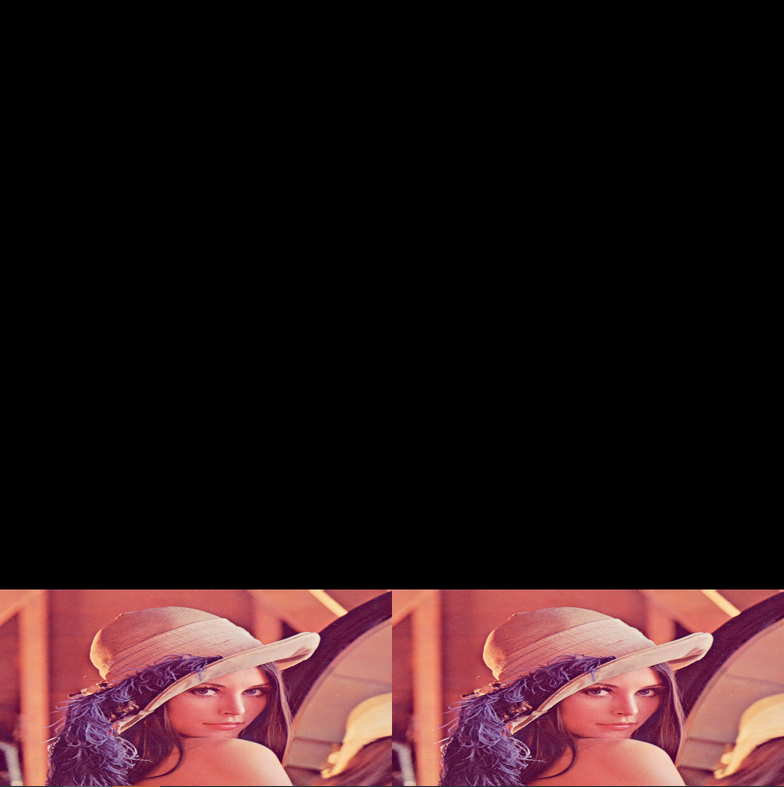
\includegraphics[scale=0.5]{imagenes/HyWmul2.png}]}
		\subfigure[Ancho y Alto dividido por 2]{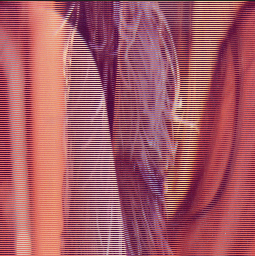
\includegraphics[scale=0.5]{imagenes/HyWdiv2.png}]
	}
	\caption{Resultado de cambiar el ancho y alto de la imagen.}
\end{figure}	

	Ahora si modifico un alto o un ancho y lo vuelvo a la normalidad se estarán perdiendo datos porque cambio la imagen  pierde los valores que se modificaron obteniendo
	
\begin{figure}[H]
	\centering
	\subfigure[Ancho y alto multiplicado por 2]{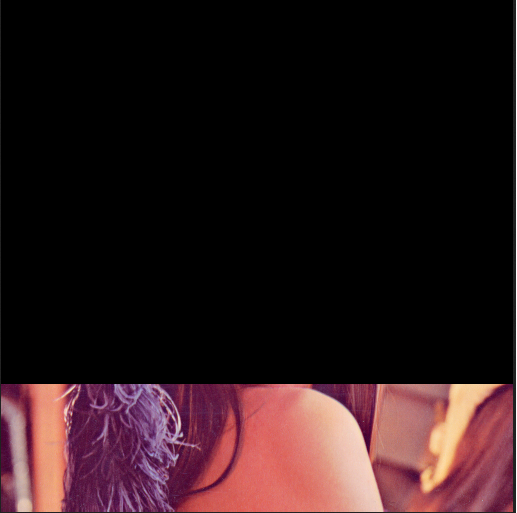
\includegraphics[scale=0.5]{imagenes/Hdiv2Yvuelvo.png}]}
		\subfigure[Ancho y Alto dividido por 2]{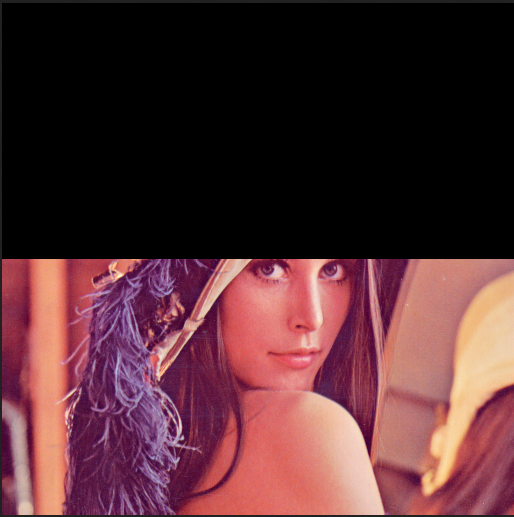
\includegraphics[scale=0.5]{imagenes/Wdiv2yVuelvo.png}]
	}
	\caption{Resultado de cambiar el ancho o alto de la imagen y volver al tamaño original.}
\end{figure}	
 
	También se modifico el valor del tamaño  de datos de la imagen, acá se hicieron varias pruebas solo modificando el tamaño y también modificando tanto el tamaño como el alto y el ancho. 

\begin{figure}[H]
	\centering
	\subfigure[Tamaño de datos dividido por 2]{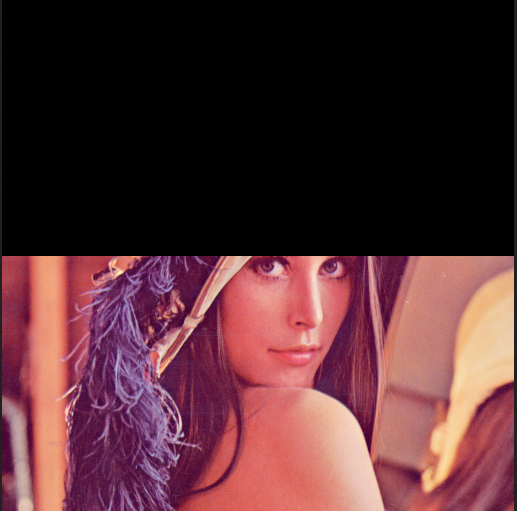
\includegraphics[scale=0.5]{imagenes/Sizediv2.png}]}
		\subfigure[Tamaño de datos multiplicado por 2 y alta y ancho de la imgen igual a 1024x1024]{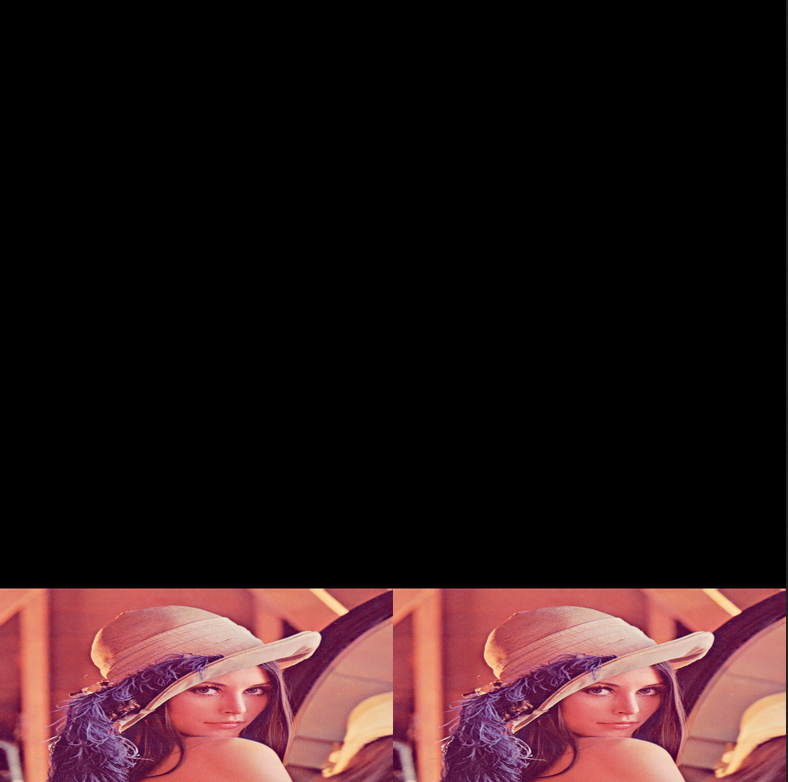
\includegraphics[scale=0.5]{imagenes/Sizemul2YHyWmul2.png}]
	}
	\caption{Resultado de cambiar el tamaño de datos de la imagen.}
\end{figure}	

Por ultimo, para el manejo del header se decidió agrandar la imagen pero en lugar de no hacer nada, se decidió copiar los datos para obtener replicas de la imagen. Para eso, se tomo el vector de datos de la imagen original y se copio tantas veces que entran en la nueva imagen obeteniendo el siguiente resultado

\begin{figure}[H]
	\centering
	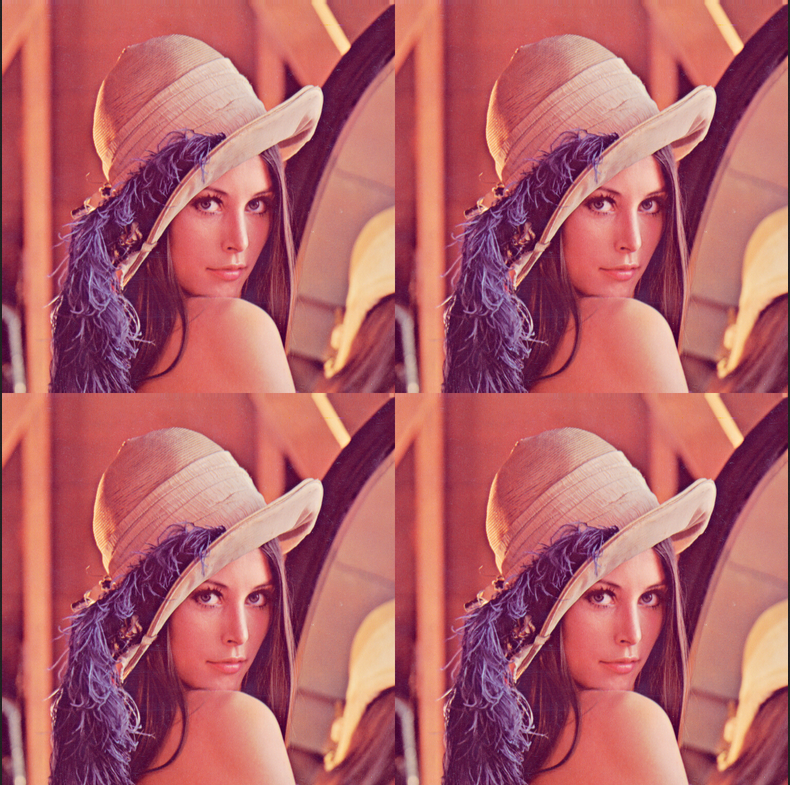
\includegraphics[scale=0.5]{imagenes/copiadoRGB.png}
	\caption{Imagen resultante del copiado de datos.}
\end{figure}

\section{Algoritmo para escala de grises}

En esta sección se tratan tres métodos para transformar la imagen \textit{lenna.bmp} a una imagen en escalas de grises. Para eso se uso un promedio de los colores RGB, también se tomo el valor del gris en RGB y por ultimo se modifico la paleta para obtener una imagen en escalas de grises. 

\subsection{Promedio de los colores RGB}

Este algoritmo consiste en tomar los valores RGB de cada pixel y hacer un promedio del mismo. Esto se puede representar como (tomando que el valor de cada pixel se divide en 3 valores RGB)

\begin{equation}
	P_{i} = \frac{R_i +G_i +B_i}{3}
\end{equation}

siendo $P_i$ el valor del nuevo pixel, por lo que se recore la imagen haciendo calculado el valor de cada nuevo pixel obteniendo 

\begin{figure}[H]
	\centering
	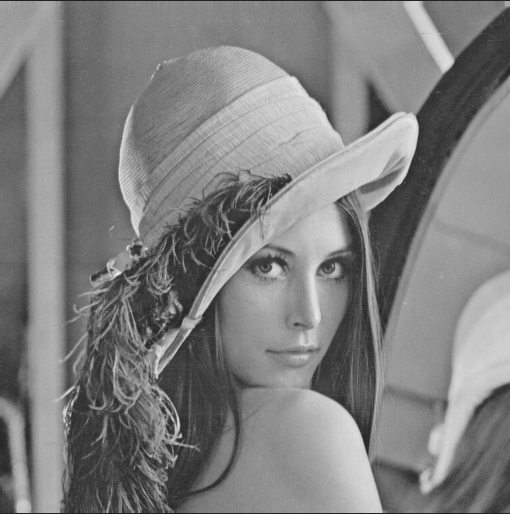
\includegraphics[scale=0.5]{imagenes/lennaGrisRGB.png}
	\caption{Imagen resultante en escala de grises.}
\end{figure}

\subsection{Valor del gris}

En este algoritmo, se busca el valor del gris en la escala RGB, y se vuelve a calcular cada pixel con respecto a este valor. El valor del nuevo pixel se puede calcular como

\begin{equation}
	P_i = 0.299 \times R + 0.587 \times G +0.144 \times B
\end{equation}

de esta forma se escala cada pixel con el color del gris, obteniendo

\begin{figure}[H]
	\centering
	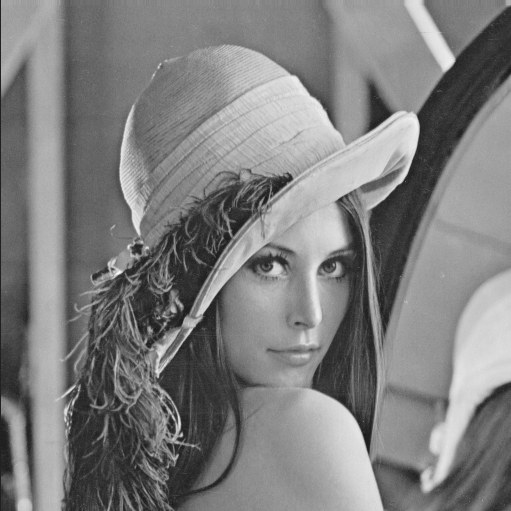
\includegraphics[scale=0.5]{imagenes/lennaGrisValores.png}
	\caption{Imagen resultante en escala de grises.}
\end{figure}

\subsection{Paleta}

La paletizacion de la imagen consiste en definir la paleta de colores en blanco y negro tomando 256 colores. La paleta en blanco y negro se define tomando la matriz y asignando la matriz de la paleta como
\begin{equation}
\begin{pmatrix}
\centering
0 & 0 & 0\\
1 & 1 & 1 \\
2 & 2 & 2 \\
\vdots & \vdots & \vdots\\
255 & 255 & 255
\end{pmatrix}
\end{equation}

el resultado de usar esta paletizacion se observa en la imagen (\ref{fig:paleta}). La idea es asignar a cada pixel el valor del promedio de la fila de la paleta, se observa que se termina haciendo algo parecido en el algoritmo del promedio de los colores RGB.

\begin{figure}[H]
	\centering
	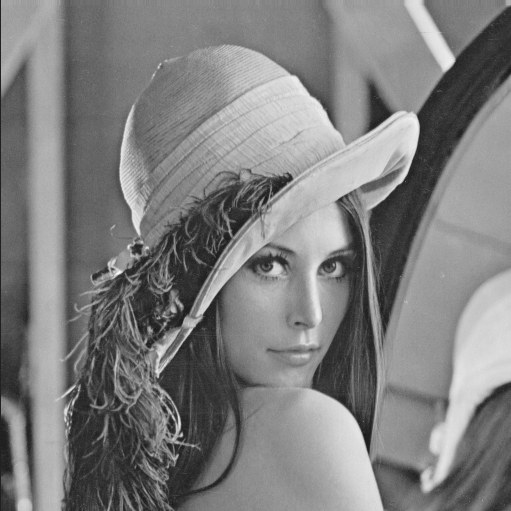
\includegraphics[scale=0.5]{imagenes/lennaGrisValores.png}
	\caption{Imagen resultante en escala de grises\label{fig:paleta}.}
\end{figure}

\section{Negativo de la imagen}

El calculo del negativo de una imagen consiste en tomar el valor valor de cada pixel de la imagen $P_i$ y calcular

\begin{equation}
P_{i,nuevo}=255-P_i
\end{equation}

donde $255$ corresponde al valor del color máximo. Así se obtiene un negativo de la imagen que corresponde al valor máximo menos el valor en ese pixel. Los resultados son
\begin{figure}[H]
	\centering
	\subfigure[Imagen negativa con lenna a color]{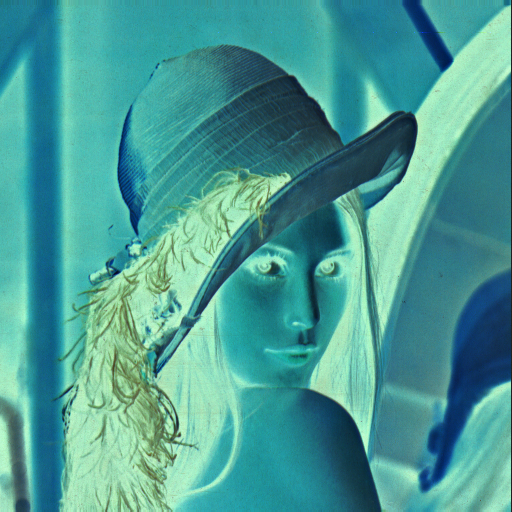
\includegraphics[scale=0.5]{imagenes/negativoColor.png}]}
		\subfigure[Imagen negativa con lenna en escala de grises]{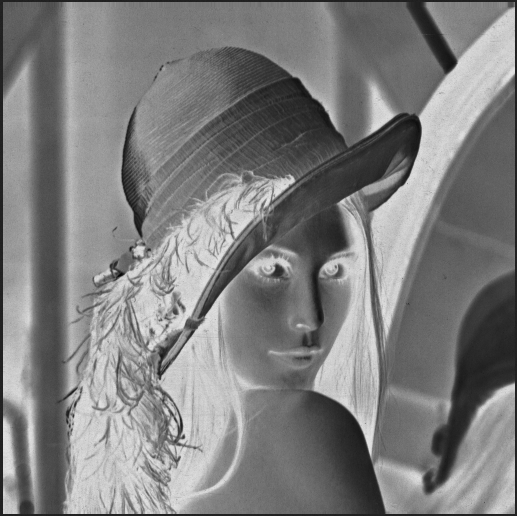
\includegraphics[scale=0.5]{imagenes/negativoGris.png}]
	}
	\caption{Resultado de la imagen negativa.}
\end{figure}	

\section{Imágenes agregando un ruido}

\subsection{Ruido constante}

Se agarro cada pixel de la imagen y se le agrego un ruido constante de valor 150. Matemáticamente seria

\begin{equation}
	P_i = P_i +150
\end{equation}

el resultado obtenido es una imagen mas clara, teniendo en cuenta que se aumenta el valor de cada pixel ahora si se reduci el valor se obtendria una imagen mas oscura. A continuación se observa la imagen resultante

\begin{figure}[H]
	\centering
	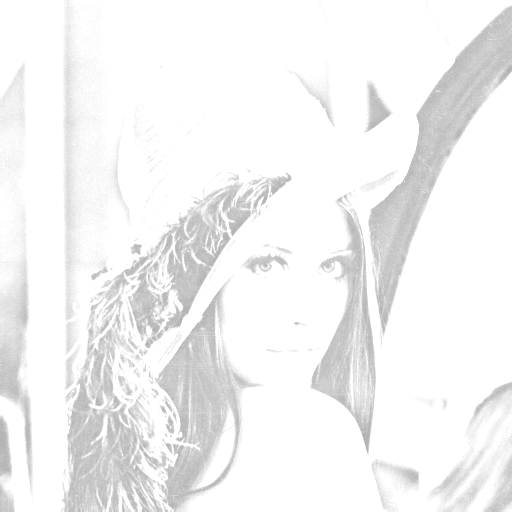
\includegraphics[scale=0.5]{imagenes/ruidoCte.png}

	\caption{Imagen resultante.}
\end{figure}	

\subsection{Ruido aleatorio con distribución Normal}

El concepto es el mismo que ruido constante solo que a cada pixel le sumo un valor generado por una densidad de probabilidad normal de media 100 y desvió 50. Al realizar esto, como la media la media es mucho mas grade que el desvió provoca que en algunos pixeles la imagen se vuelva mas clara que en otros.


\begin{figure}[H]
	\centering
	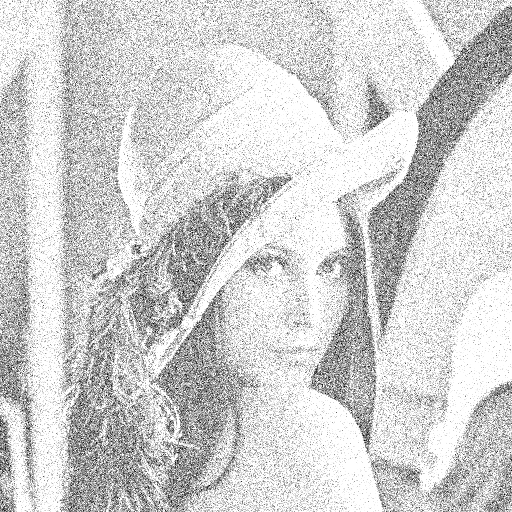
\includegraphics[scale=0.5]{imagenes/ruidoAleatorioNormal.png}

	\caption{Imagen resultante.}
\end{figure}

\subsection{Ruido Aleatorio con distribución Bernulli}

Al igual que en el caso anterior, se tomo el valor de cada pixel y se lo sumo con valores generados por una densidad bernulli generando 1 o 0, que luego se multiplica por un valor de 100 obteniendo que algunos pixeles se suen con este valor y otros que no sumen nada.

\begin{figure}[H]
	\centering
	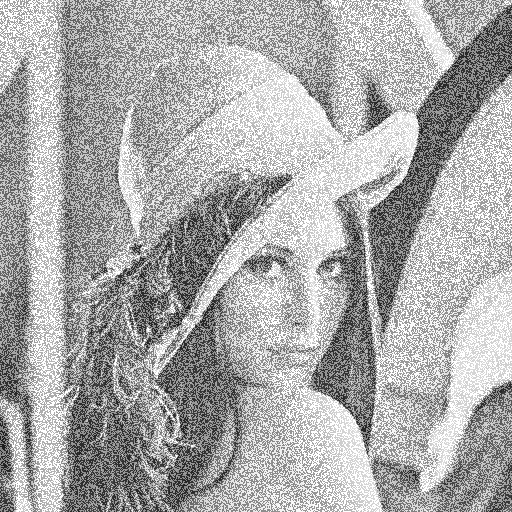
\includegraphics[scale=0.5]{imagenes/ruidoAleatorioBernuli.png}

	\caption{Imagen resultante.}
\end{figure}

\section{Recorrido de una imagen}

Existen diferentes métodos para recorrer una imagen, entre ellos los dos mas conocidos son el horizontal y el vertical para los cuales se calculo la diferencia entre los pixeles para obtener el contorno de la imagen. Luego, se realizo el recorrido de la imagen con un recorrido conocido como Hilbert. 

\section{Recorrido horizontal y vertical}


En la figura (\ref{fig:recorrido}), muestra la forma de ambos recorrido. Considerando a la imagen como un matriz, cada recorrido se puede definir como van variando el paso de esta matriz, esto seria que para el recorrido horizontal se mantengo fija la fila  me muevo por las columnas mientras que para el recorrido vertical mantengo fijo las columnas y me muevo por las filas. 

\begin{figure}[H]
	\centering
	\subfigure[Recorrido horizontal.]{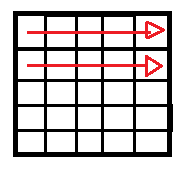
\includegraphics[scale=0.75]{imagenes/recoridoH.png}}
		\subfigure[Recorrido vertical]{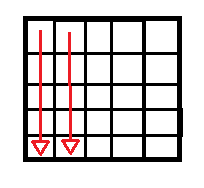
\includegraphics[scale=0.75]{imagenes/recorridoV.png}}
\end{figure}	

Teniendo en cuenta el valor de cada pixel, se realizo los dos recorridos con el propósito de buscar un contorno de la imagen, tomando la diferencia en cada pixel y preguntando si era mayor a un cierto umbral. El mismo se mantuvo fijo para ambos recorridos, luego se realizo el histograma sobre la diferencia de los pixeles obteniendo valores muy pequeños o valores muy grandes, teniendo en cuento que la diferencia entre pixel es muy grande cuando hay un borde.

\begin{figure}[H]
	\centering
	\subfigure[Contorno con recorrido horizontal.]{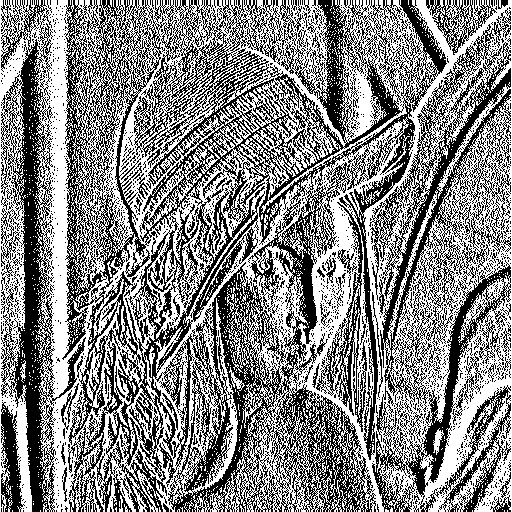
\includegraphics[scale=0.5]{imagenes/recorridoHorizontal.png}}
		\subfigure[Contorno con recorrido vertical]{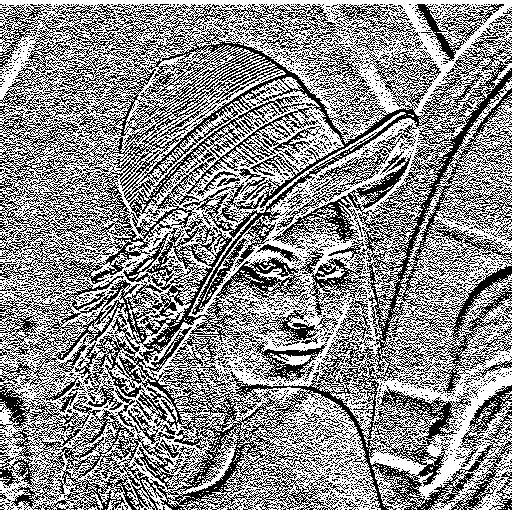
\includegraphics[scale=0.5]{imagenes/recoridoVertical.png}}
	\caption{Resultados de ambos recorridos}
\end{figure}	



\begin{figure}[H]
	\centering
	\subfigure[Histograma con recorrido horizontal.]{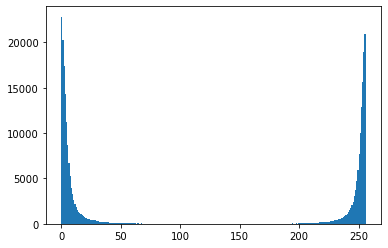
\includegraphics[scale=0.5]{imagenes/recorridoHorizontal-Histograma.png}]}
		\subfigure[Histograma con recorrido vertical]{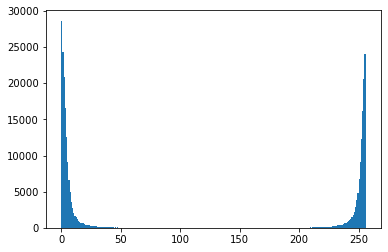
\includegraphics[scale=0.5]{imagenes/recorridoVertical-Histograma.png}]
	}
	\caption{Histograma de ambos recorridos}
\end{figure}	

	Se observa que al cambiar el recorrido aparecen diferentes contornos en distintas orientaciones.Para finalizar se realizo la suma de las imagen del contorno obteniendo, esto provoa que la imagen se vuelva mas clara en algunos lugares oscuro haciendo notar mas el contorno.
	
\begin{figure}[H]
	\centering
	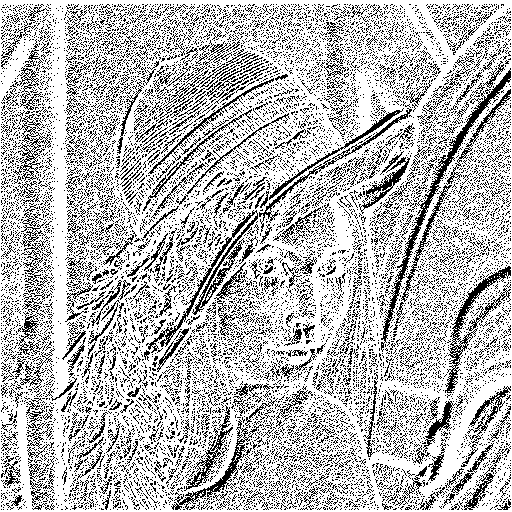
\includegraphics[scale=0.5]{imagenes/sumaRecorido.png}

	\caption{Imagen resultante.}
\end{figure}

\section{Recorrido de Hilbert}

El recorrido de Hilbert consiste en ir variando la fila o la columna a continuar a través de unas curvas conocidas como curvas de Hilbert. En la figura (\ref{fig:curvas-Hilbert}) se muestran las diferentes curvas, en donde se generan las curvas a través de la primer imagen de la figura, la cual va variando la orientación y se va uniendo para formas otros tipos de curvas.

\begin{figure}[H]
	\centering
	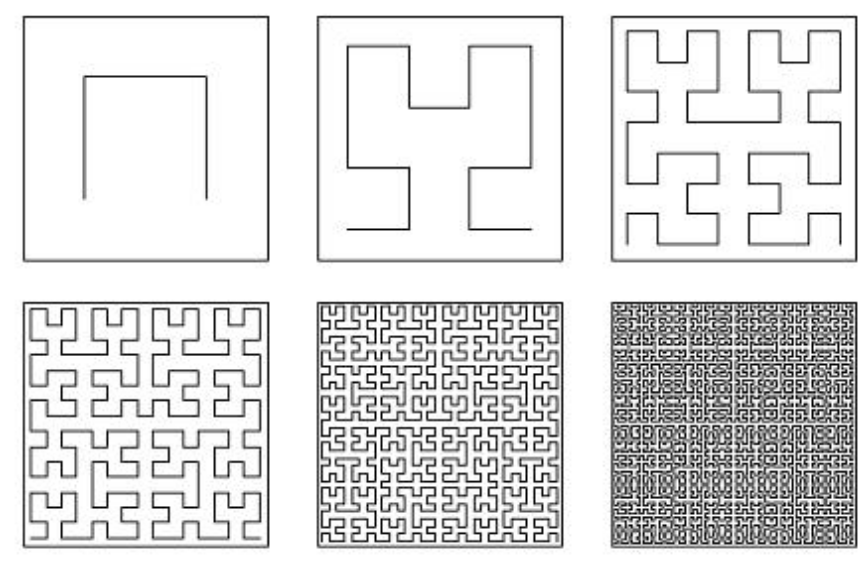
\includegraphics[scale=0.5]{imagenes/curvasHilbert.png}

	\caption{Curvas de Hilbert\label{fig:curvas-Hilbert}.}
\end{figure}

Entonces se tomo la imagen de lena y se realizo el recorrido. la figura (\ref{fig:hilbert}) muestra la imagen patrón con el recorrido realizado sobre la misma imagen.

\begin{figure}[H]
	\centering
	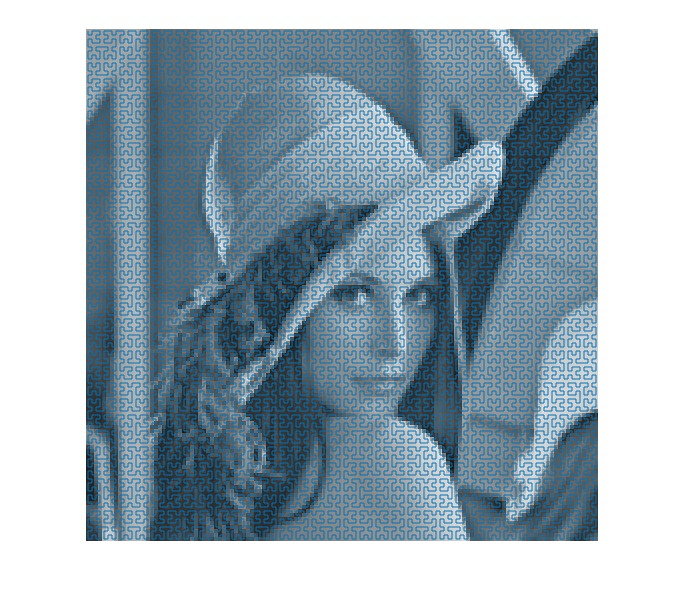
\includegraphics[scale=0.5]{imagenes/hilbert.jpeg}

	\caption{Recorrido de Hilbert\label{fig:hilbert}.}
\end{figure}

\section{Zoom}

	El \textit{Zoom} de una imagen consiste en agarrar los datos de los pixel y duplicarlo en los pixeles de alrededor. La figura (\ref{fig:zoom}) muestra el proceso de agrandamiento de una imagen, se ve que se toma cada pixel y multiplicarlo por una matriz de todos 1 para duplicar el pixel, luego se guarda en otra imagen de mayor tamaño o igual.
	

\begin{figure}[H]
	\centering
	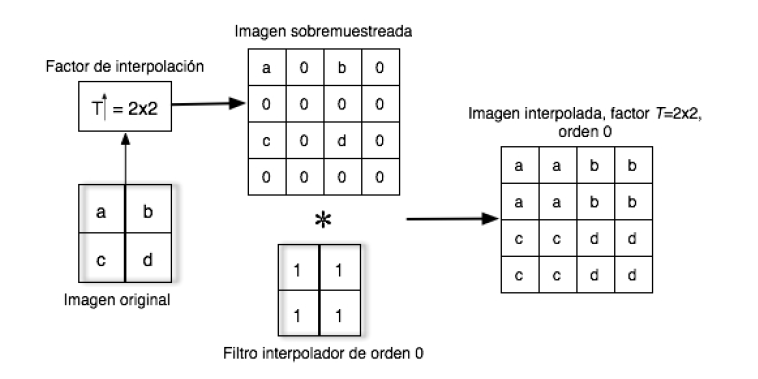
\includegraphics[scale=0.5]{imagenes/zoom0-sis.png}

	\caption{Recorrido de Hilbert\label{fig:zoom}.}
\end{figure}

Por lo tanto, se dividió la imagen en 4 partes iguales tomando un tamaño de 256x256, luego se agrando cada una de estas partes a una nueva imagen de 512x512 obteniendo

\begin{figure}[H]
	\centering
	\subfigure{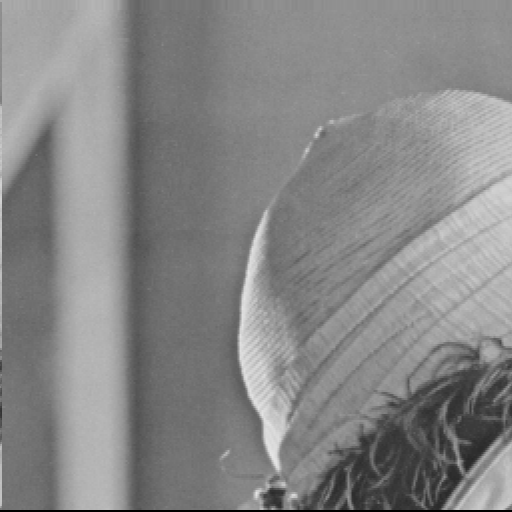
\includegraphics[scale=0.4]{imagenes/sup-izqZoom0.png}]}
		\subfigure{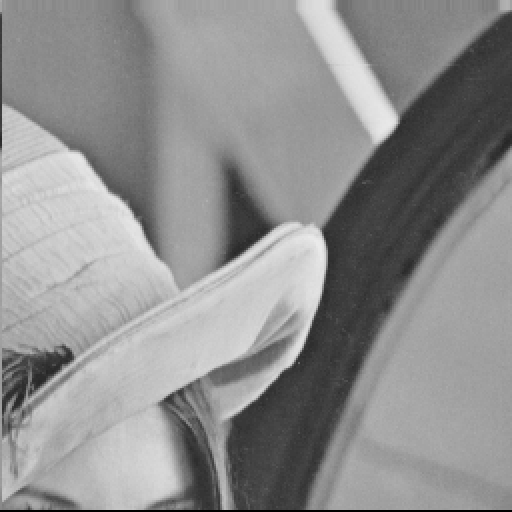
\includegraphics[scale=0.4]{imagenes/sup-derZoom0.png}]}
		\subfigure{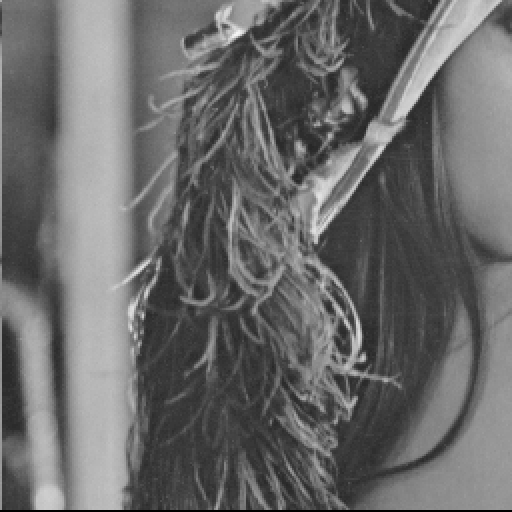
\includegraphics[scale=0.4]{imagenes/inf-izqZoom0.png}]}
		\subfigure{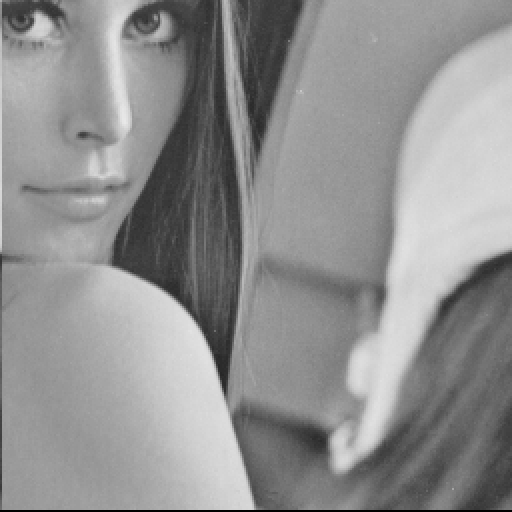
\includegraphics[scale=0.4]{imagenes/inf-derZoom0.png}]}
	\caption{Zoom de la imagen original}
\end{figure}

\section{Transformada Coseno}

A partir de la imagen se decidio calcular la transformada coseno de a imagen. Luego, en la figura (\ref{fig:tc}) se observa el histograma rojo correspondiente a la transformada coseno y el histograma verde correspondiente a la imagen original. Al realizar la transformada coseno se observa como la energía de la imagen se concentra en los primeros valores de los pixeles, mientras que en el histograma original los concentra sobre todos los pixeles. 

\begin{figure}[H]
	\centering
	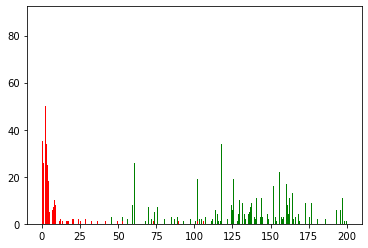
\includegraphics[scale=0.5]{imagenes/transformadaCoseno.png}

	\caption{Transformada coseno \label{fig:tc}.}
\end{figure}

Por lo tanto, se podría usar la transformada coseno para comprimir la imagen ya que me guarda la información en los primeros pixeles, permitiendo dejar de considerar los siguientes pixeles.

\section{Ecualización del histograma}

	La ecualización del histograma de una imagen consiste en una transformación del histograma. Una imagen tendrá un cierto histograma que depende de los valores de los pixeles, en la ecualización del histograma se intenta hacer que el resultado sea un histograma uniforme con respecto al original. La figura (\ref{fig:ec}) muestra el histograma de la figura original poco uniforme con el histograma después de la ecualización que intenta tender a una uniformidad. Por otro lado, la imagen (\ref{fig:ecImg}) muestra la imagen resultante después de la ecualización, se puede observar un aumento en la resolución de la imagen original. Para realizar la ecualización, se uso una función de ecualización que transforma el valor de cada pixel al valor de la imagen resultante, el sistema completo se puede ver en la siguiente imagen

\begin{figure}[H]
	\centering
	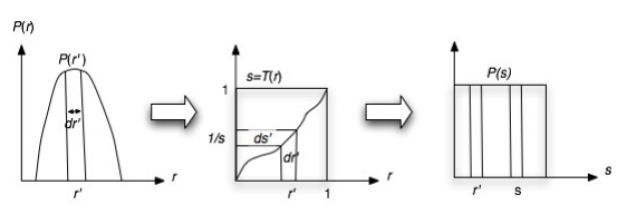
\includegraphics[scale=0.5]{imagenes/ecSis.png}

	\caption{Sistema de ecualización del histograma\label{fig:ecSis}.}
\end{figure}

donde se puede observar claramente que la función que transforma el histograma es la función $T(f)$ logrando la uniformidad del mismo.

\begin{figure}[H]
	\centering
	\subfigure[Histograma de la imagen original.]{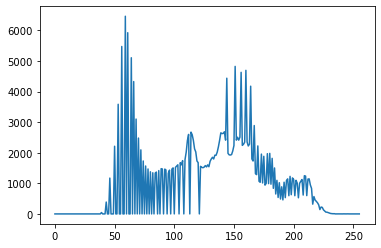
\includegraphics[scale=0.5]{imagenes/histOriginal.png}]}
		\subfigure[Histograma con recorrido vertical]{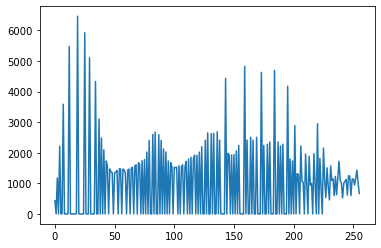
\includegraphics[scale=0.5]{imagenes/histEcualizado.png}]
	}
	\caption{Histograma original y ecualizado \label{fig:ec}}
\end{figure}	

\begin{figure}[H]
	\centering
	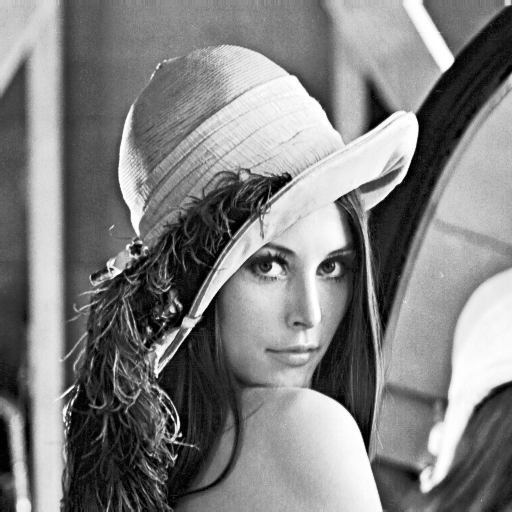
\includegraphics[scale=0.5]{imagenes/ecualidazorHistograma.png}

	\caption{Imagen resultante histograma ecualizado\label{fig:ecImg}.}
\end{figure}

\section{Streching}

	El Streching es un método para la ecualización del histograma con la diferencia que se asigna los valores de las porciones mas que ocurren de los rangos del histograma y menos de visualización a la menor frecuencia de los valores de brillo. Este método de realce espectral reduce el contraste que se pueda presentar entre aquellas áreas muy claras o muy oscuras de una imagen con una distribución mas alargada de los extremos mínimos y máximos de un histograma, por lo que se tomara el valor máximo y mínimo de la imagen para realizar la operación de Streching, se calcula el valor de cada pixel de nuevo a traves de 
\begin{equation}
	p_i = 255 \times \frac{p_i-p_{min}}{p_{max}-p_{min}}
\end{equation}
en donde $p_{min}$ y $p_{max}$ representa el valor de los pixeles máximo y mínimo de la imagen. Al realizar esto logramos aumentar la resolución como se observa a continuación

\begin{figure}[H]
	\centering
	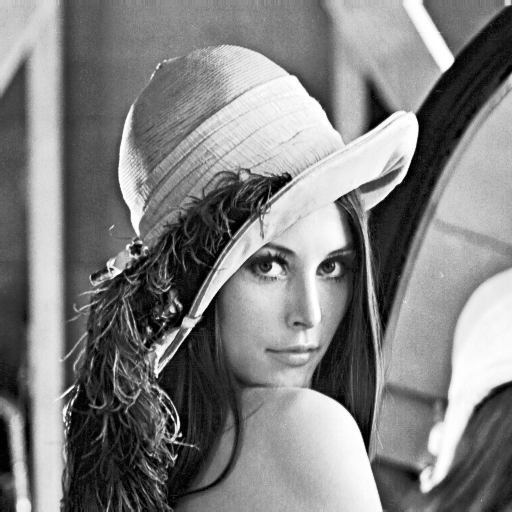
\includegraphics[scale=0.5]{imagenes/stretching.png}

	\caption{Stretching\label{fig:st}.}
\end{figure}


\section{Compresión}

Un problema en la codificación de datos es la compresión de los datos para ahorrar espacio en la computadora sin perder la información de los datos, para eso se usan diferentes herramientas para la codificación de los datos, en este trabajo realizaremos una compresión a través de un algoritmo no supervisado variando la cantidad de clases, y mencionaremos otro método de compresión conocido como \textit{IFS}

\subsection{K-means}

	El algoritmo de \textit{k-means} es un algoritmo no supervisado que calcula las clases a partir de las media de cada una de ellas y busca minimizar la distancia entre los datos y las clases para determinar al clusters que pertenece. Tenes en cuanta que en una imagen, las clases serian los valores de los pixeles por ende cuando menos clases tengo mas diferencia con la imagen original tengo hasta un valor de 255 que asigna una clase a cada pixel. En la siguiente figura se observa eso, se tomaron una cantidad de clases K igual a $5,10,20,40,80,100 y 255$ para ver los cambios que ocurren al momento de aumentar la cantidad de clases, se puede observar que con un $K=5$ se pierde la resolución de la imagen y a medida que se aumenta la cantidad de las clases empieza a mejorar hasta un punto que no se puede notar una diferencia con la imagen original. 

\begin{figure}[H]
	\centering
	\subfigure[k=5]{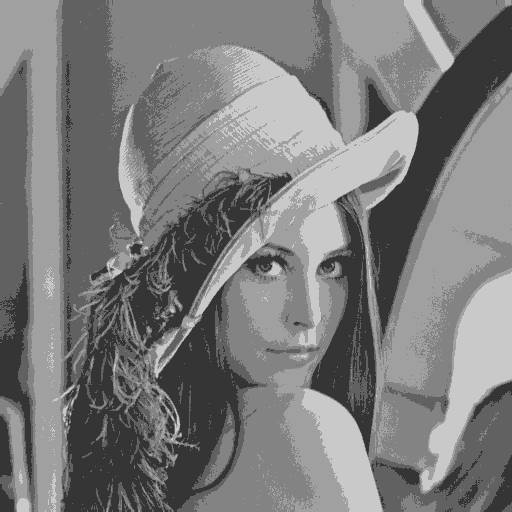
\includegraphics[scale=0.25]{imagenes/kmeans-k-5.png}]}
		\subfigure[k=10]{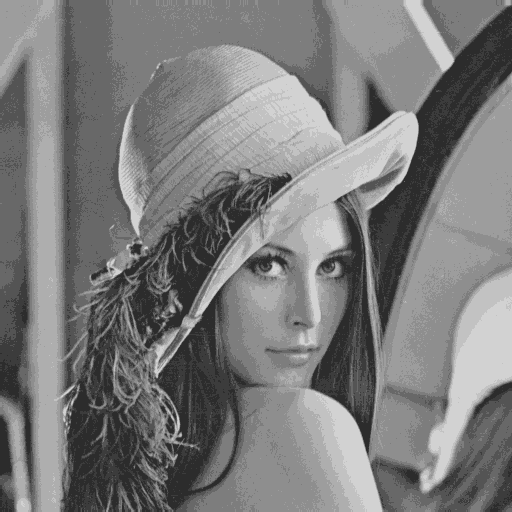
\includegraphics[scale=0.25]{imagenes/kmeans-k-10.png}]}
		\subfigure[k=20]{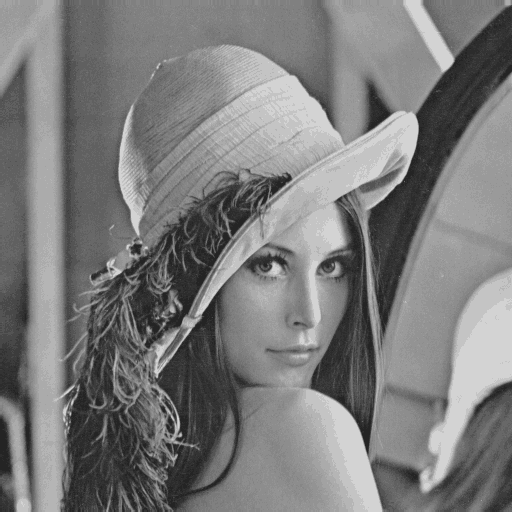
\includegraphics[scale=0.25]{imagenes/kmeans-k-20.png}]}
		\subfigure[k=40]{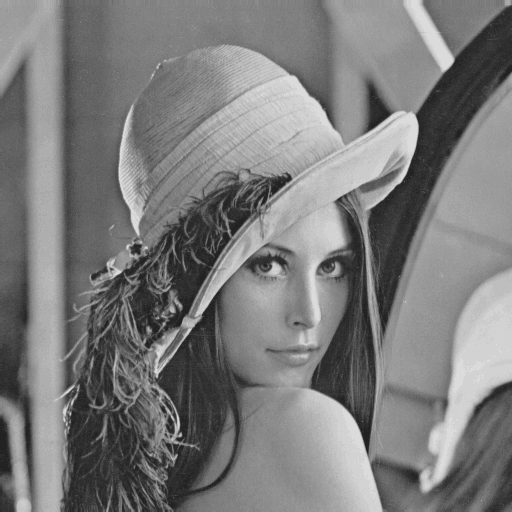
\includegraphics[scale=0.25]{imagenes/kmeans-k-40.png}]}
		\subfigure[k=80]{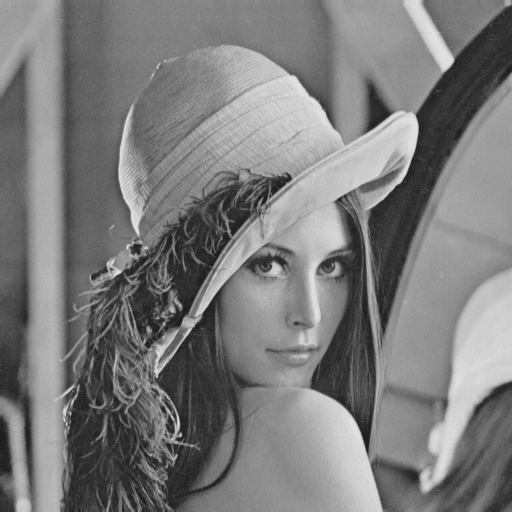
\includegraphics[scale=0.25]{imagenes/kmeans-k-80.png}]}
		\subfigure[k=100]{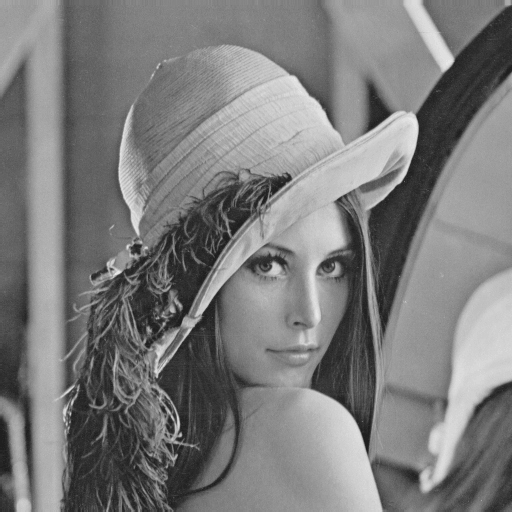
\includegraphics[scale=0.25]{imagenes/kmeans-k-100.png}]}
		\subfigure[k=255]{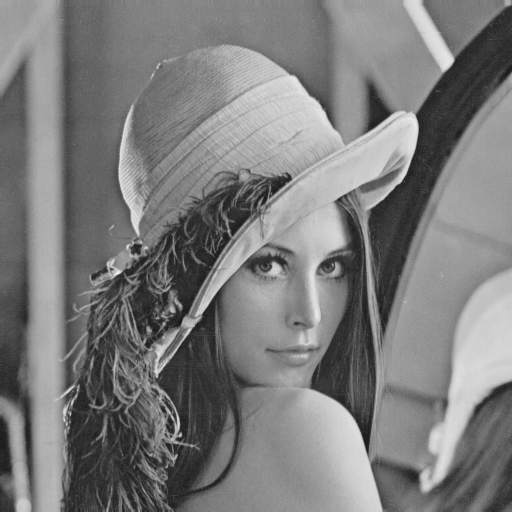
\includegraphics[scale=0.25]{imagenes/kmeans-k-255.png}]}
	\caption{Compresión con el algoritmo k-means}
\end{figure}

Es importante destacar, que en una imagen puede ocurrir que no se usen los 255 pixeles por lo que al realizar la compresion de la misma no se observa ninguna diferencia. Por ejemplo, si uso una imagen que use solo 5 pixeles, entonces la compresión con una clase $K=5$ no habrá diferencia entre la imagen original porque cada pixel tendrá su clase determinado.


\subsection{IFS}

	El método \textit{IFS} consiste en una compresión fractal teniendo mejor resultados para texturas y imagen naturales. Se usa sistemas de funciones iterativo que es un método para construir los fractal. La idea es ir generando los fractal y ir uniendolos como se muestra en la figura (\ref{fig:IFS}), mostrando como se unen los cuadrados con diferentes orientacion.
	
\begin{figure}[H]
	\centering
	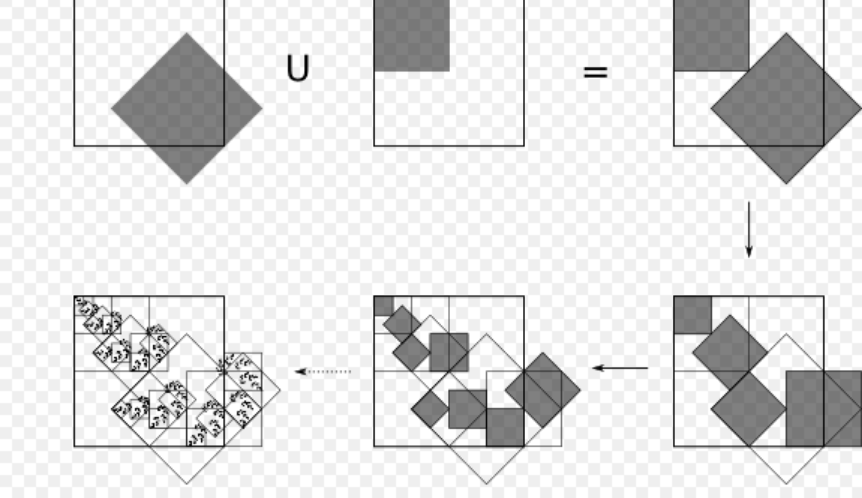
\includegraphics[scale=0.5]{imagenes/IFS.png}

	\caption{IFS\label{fig:IFS}.}
\end{figure} 

Basicamente, la compresion de IFS consiste en un mapero en una dimension $\mathbb{R}^N$ a $\mathbb{R}^N$. En imágenes, se puede tener imágenes binarias o imágenes ternarias obteniendo transformacion$f_i:\mathbb{R}^2\longrightarrow\mathbb{R}^2$ o $f_i:\mathbb{R}^3\longrightarrow\mathbb{R}^3$. Por lo que la idea del mapeo seria obtener un operador de la forma

\begin{equation}
H(A)=\cup^N_{i=1}f_i(A),\;A\subset\mathbb{R}
\end{equation}

observando que se van uniendo los fractal como se mostraba en la imagen, el valor de A permite la rotación del fractal. Generalmente, en escala de grises se usa un $\mathbb{R}^3$ con un conjunto de fractal $S={(x,y,u(x,y))}$ siendo $u(x,y)$ los valores en escala de grises, es la misma idea que antes tengre funciones $f_1,...,f_N$ pero ahora en $\mathbb{R}^3$.